\documentclass[12pt]{iopart} % Document class declaration

% package "imports"
\usepackage{graphicx}
\usepackage{IEEEtrantools}

% Custom macros
\gdef\mcm{r@{.}l@{ ± }r@{.}l} % Multi Column Measurement; Used for decimal aligning & ± aligning
\gdef\mch#1{\multicolumn{4}{l}{#1}} % Multi Column Header; Used for decimal aligning & ± aligning
\gdef\mcmnd{r@{ ± }l} % Multi Column Measurement No Decimal; Used for ± aligning when the values don't need a decimal point
\gdef\mchnd#1{\multicolumn{2}{l}{#1}} % Multi Column Header No Decimal; Used for  ± aligning when the values don't need a decimal point
\gdef\sci#1#2{#1 \times 10^{#2}}
\gdef\units#1{~\mathrm{#1}}

%%%%%%%%%%%%%%%%%%%% Document Starts %%%%%%%%%%%%%%%%%%%%
\begin{document}

%%%%%%%%%%%%%%%%%%%% Title Page %%%%%%%%%%%%%%%%%%%%
\title{Carnot Cycle Exercise}
\author{Vincent Edwards}
\vspace{10pt}
\begin{indented}
  \item[]Mt.~San Antonio College, Physics 4B, CRN 42240
  \item[]March 27, 2023
  \item[]
  \item[]$T_H = 490~\mathrm{K}$
  \item[]$V_c = \sci{1.90}{-3} \units{m^3}$
\end{indented}
\newpage

%%%%%%%%%%%%%%%%%%%% Purpose %%%%%%%%%%%%%%%%%%%%
\section{Purpose}

The goal of the exercise is to perform various calculations related to the Carnot cycle.

%%%%%%%%%%%%%%%%%%%% Given %%%%%%%%%%%%%%%%%%%%
\section{Given}

\begin{itemize}
  \item $T_H = 490 \units{K}$
  \item $T_C = 300 \units{K}$
  \item $P_c = \sci{1.01}{5} \units{Pa}$
  \item $V_c = \sci{1.90}{-3} \units{m^3}$
  \item $Q_{a \to b} = 300 \units{J}$
  \item $\gamma = 1.40$
  \item $\mathrm{d.o.f.} = 5$
  \item $C_v = \frac 5 2 R$
  \item $C_p = \frac 7 2 R$
\end{itemize}

%%%%%%%%%%%%%%%%%%%% Derivations %%%%%%%%%%%%%%%%%%%%
\section{Derivations}

\subsection{Pressure--Volume Relationship for Adiabatic Process}

\begin{IEEEeqnarray*}{rCl}
  \Delta U & = & Q - W \\
  \Delta U & = & - W \\
  d U & = & - dW \\
  n C_v dT & = & - P dV \\
  n dT & = & - \frac{P dV}{C_v}
\end{IEEEeqnarray*}

\begin{IEEEeqnarray*}{rCl}
  P V & = & n R T \\
  P dV + V dP & = & n R dT \\
  P dV + V dP & = & (C_p - C_v) n dT \\
  P dV + V dP & = & - (C_p - C_v) \frac{P dV}{C_v} \\
  P dV + V dP & = & \left(1 - \frac{C_p}{C_v} \right) P dV \\
  V dP & = & - \frac{C_p}{C_v} P dV \\
  V dP & = & - \gamma P dV \\
  \frac{dP}{P} & = & - \gamma \frac{dV}{V} \\
  \int\frac{dP}{P} & = & -\int\gamma \frac{dV}{V} \\
  \ln(P) & = & -\gamma \ln(V) + \mathrm{const.} \\
  \ln(P) + \ln(V^\gamma) & = & \mathrm{const.} \\
  \ln(P V^\gamma) & = & \mathrm{const.} \\
  P V^\gamma & = & \mathrm{const.} \\
  P_i V_i^\gamma & = & P_f V_f^\gamma
\end{IEEEeqnarray*}

\subsection{Temperature--Volume Relationship for Adiabatic Process}

\begin{IEEEeqnarray*}{rCl}
  P_i V_i^\gamma & = & P_f V_f^\gamma \\
  P_i V_i V_i^{\gamma-1} & = & P_f V_f V_f^{\gamma-1} \\
  n R T_i V_i^{\gamma-1} & = & n R T_f V_f^{\gamma-1} \\
  T_i V_i^{\gamma-1} & = & T_f V_f^{\gamma-1} 
\end{IEEEeqnarray*}

\subsection{Work by Gas for Isothermal Process}

\begin{IEEEeqnarray*}{rCl}
  W & = & \int\limits_{i \to f} P dV \\
  W & = & \int\limits_{V_i}^{V_f} \frac{nRT}{V} dV \\
  W & = & nRT \ln(V) \vert_{V_i}^{V_f} \\
  W & = & nRT (\ln(V_f) - \ln(V_i)) \\
  W & = & nRT \ln\left( \frac{V_f}{V_i} \right)
\end{IEEEeqnarray*}

\subsection{Work by Gas for Adiabatic Process}

\begin{IEEEeqnarray*}{rCl}
  W & = & \int\limits_{i \to f} P dV \\
  W & = & \int\limits_{V_i}^{V_f} (P_i V_i^\gamma) V^{-\gamma} dV \\
  W & = & \frac{P_i V_i^\gamma}{1-\gamma} V^{1-\gamma} \vert_{V_i}^{V_f} \\
  W & = & \frac{P_i V_i^\gamma}{1-\gamma} (V_f^{1-\gamma} - V_i^{1-\gamma}) \\
  W & = & \frac{P_i V_i^\gamma V_f^{1-\gamma} - P_i V_i^\gamma V_i^{1-\gamma}}{1-\gamma} \\
  W & = & \frac{P_f V_f^\gamma V_f^{1-\gamma} - P_i V_i^\gamma V_i^{1-\gamma}}{1-\gamma} \\
  W & = & \frac{P_f V_f - P_i V_i}{1-\gamma} \\
  W & = & \frac{P_i V_i - P_f V_f}{\gamma-1}
\end{IEEEeqnarray*}

\subsection{Carnot Cycle Heat Ratio Equals Temperature Ratio}

\begin{IEEEeqnarray*}{rClrCl}
  \Delta U_{a \to b} & = & Q_{a \to b} - W_{a \to b} \\
  0 & = & Q_H - nRT_H \ln\left( \frac{V_b}{V_a} \right) \\
  Q_H & = & nRT_H \ln\left( \frac{V_b}{V_a} \right)
\end{IEEEeqnarray*}
\begin{IEEEeqnarray*}{rCl}
  \Delta U_{c \to d} & = & Q_{c \to d} - W_{c \to d} \\
  0 & = & Q_C - nRT_C \ln\left( \frac{V_d}{V_c} \right) \\
  Q_C & = & nRT_C \ln\left( \frac{V_d}{V_c} \right) \\
  Q_C & = & -nRT_C \ln\left( \frac{V_c}{V_d} \right)
\end{IEEEeqnarray*}
\begin{IEEEeqnarray*}{rCl}
  \frac{Q_H}{Q_C} & = & \frac{nRT_H \ln(V_b / V_a )}{-nRT_C \ln( V_c / V_d )} \\
  -\frac{Q_H}{Q_C} & = & \frac{T_H \ln(V_b / V_a )}{T_C \ln( V_c / V_d )}
\end{IEEEeqnarray*}

\begin{IEEEeqnarray*}{rCl}
  T_b V_b^{\gamma-1} & = & T_c V_c^{\gamma-1} \\
  \frac{T_b}{T_c} & = & \left( \frac{V_c}{V_b} \right)^{\gamma-1} \\
  \frac{T_H}{T_C} & = & \left( \frac{V_c}{V_b} \right)^{\gamma-1}
\end{IEEEeqnarray*}
\begin{IEEEeqnarray*}{rCl}
  T_a V_a^{\gamma-1} & = & T_d V_d^{\gamma-1} \\
  \frac{T_a}{T_d} & = & \left( \frac{V_d}{V_a} \right)^{\gamma-1} \\
  \frac{T_H}{T_C} & = & \left( \frac{V_d}{V_a} \right)^{\gamma-1}
\end{IEEEeqnarray*}
\begin{IEEEeqnarray*}{rCl}
  \left( \frac{V_c}{V_b} \right)^{\gamma-1} & = & \left( \frac{V_d}{V_a} \right)^{\gamma-1} \\
  \frac{V_c}{V_b} & = & \frac{V_d}{V_a} \\
  \frac{V_c}{V_d} & = & \frac{V_b}{V_a} \\
  \ln\left( \frac{V_c}{V_d} \right) & = & \ln\left( \frac{V_b}{V_a} \right) \\
  1 & = & \frac{\ln(V_b / V_a )}{\ln( V_c / V_d )}
\end{IEEEeqnarray*}

\begin{IEEEeqnarray*}{rCl}
  -\frac{Q_H}{Q_C} & = & \frac{T_H \ln(V_b / V_a )}{T_C \ln( V_c / V_d )} \\
  -\frac{Q_H}{Q_C} & = & \frac{T_H}{T_C} \\
  \left| -\frac{Q_H}{Q_C} \right| & = & \left| \frac{T_H}{T_C} \right| \\
  \frac{|Q_H|}{|Q_C|} & = & \frac{T_H}{T_C} \\
  \frac{T_C}{T_H} & = & \frac{|Q_C|}{|Q_H|}
\end{IEEEeqnarray*}

%%%%%%%%%%%%%%%%%%%% Results %%%%%%%%%%%%%%%%%%%%
\section{Results}

Table \ref{tab:state_variables_key_points} contains the values for pressure, volume, and temperature at the key points of the Carnot cycle.
Table \ref{tab:process_variables} contains the values for heat transferred, work done, change in internal energy, and change in entropy for the key processes.
Table \ref{tab:pv_diagram_points} contains the pressure and volume points plotted on figure \ref{fig:pv_diagram}, the $PV$-diagram for the process.
Figure \ref{fig:ts_diagram} is the $TS$-diagram for the process.
Various calculations are shown in the subsections below.

\begin{table}[htbp]
\caption{\label{tab:state_variables_key_points}
Pressure, Volume, and Temperature for Key Points \\
Note: $T_a = T_b = T_H$ and $T_c = T_d = T_C$
}
\begin{indented}\lineup\item[]\begin{tabular}{llll}
\br
Point & $P$ (Pa) & $V \units{(m^3)}$ & $T$ (K) \\
\mr
a & $\sci{1.46}{6}$ & $\sci{2.14}{-4}$ & 490 \\
b & $\sci{5.62}{5}$ & $\sci{5.57}{-4}$ & 490 \\
c & $\sci{1.01}{5}$ & $\sci{1.90}{-3}$ & 300 \\
d & $\sci{2.63}{5}$ & $\sci{7.30}{-4}$ & 300 \\
\br
\end{tabular}\end{indented}\end{table}

\begin{table}[htbp]
\caption{\label{tab:process_variables}
Heat Transferred, Work Done, Change in Internal Energy, and Change in Entropy for Key Processes \\
Note: $Q_{a \to b} = Q_H$ and $Q_{c \to d} = Q_C$
}
\begin{indented}\lineup\item[]\begin{tabular}{llllll}
\br
Process & Type & $Q$ (J) & $W$ (J) & $\Delta U$ (J) & $\Delta S$ (J/K) \\
\mr
$a \to b$ & isothermal expansion   & 300  &  300 &  0   &  0.612 \\
$b \to c$ & adiabatic expansion    & 0    &  304 &\-304 &  0     \\
$c \to d$ & isothermal compression &\-184 &\-184 &  0   &\-0.612 \\
$d \to a$ & adiabatic compression  & 0    &\-304 &  304 &  0     \\
Total     & Carnot cycle           & 116  &  116 &  0   &  0     \\
\br
\end{tabular}\end{indented}\end{table}

\begin{figure}[htbp]
  \begin{indented}
  \item[]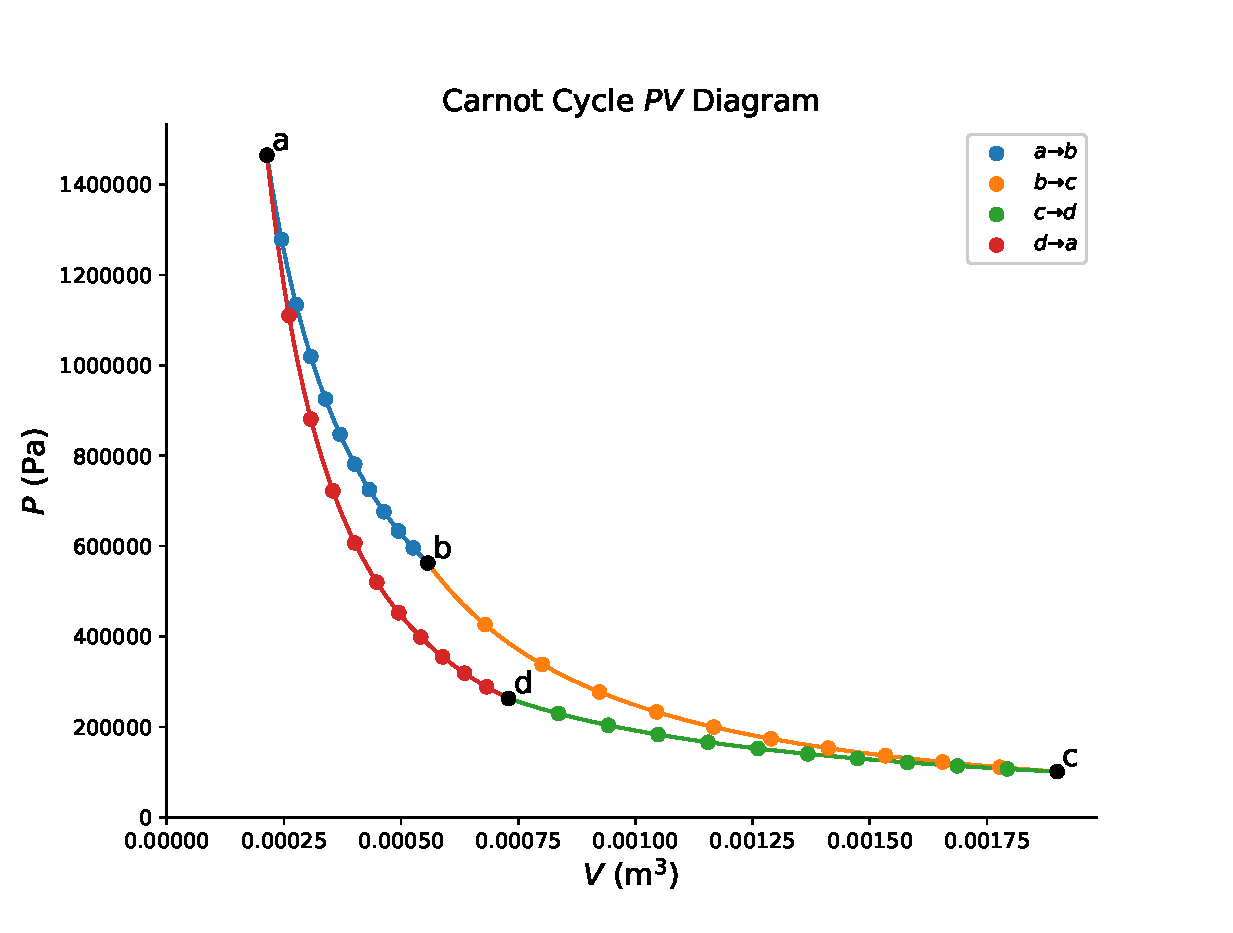
\includegraphics[width=0.83\textwidth]{pv-diagram-carnot-cycle.eps}
  \end{indented}
  \caption{\label{fig:pv_diagram}
  Carnot Cycle $PV$-Diagram
  }
\end{figure}

\begin{figure}[htbp]
  \begin{indented}
  \item[]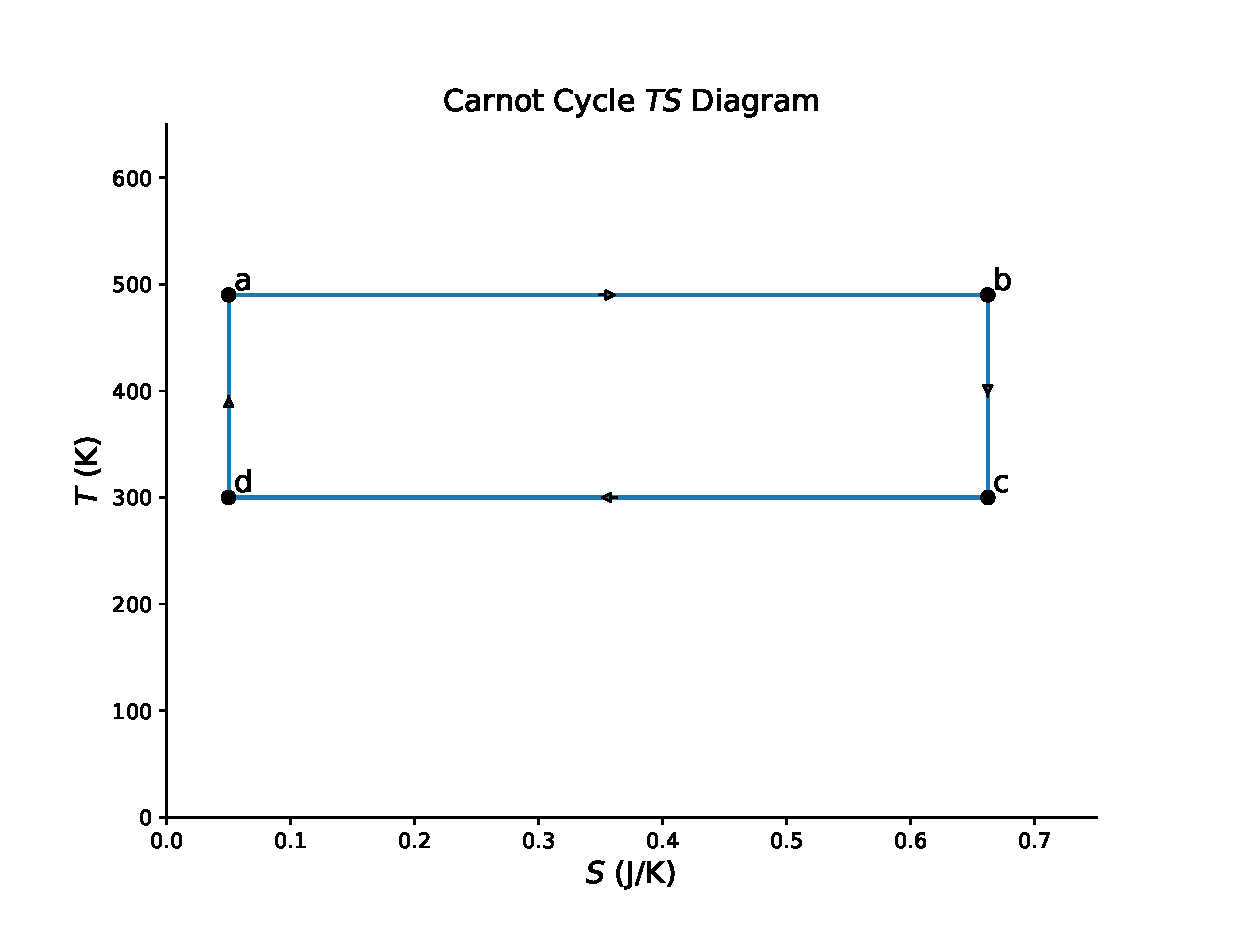
\includegraphics[width=0.83\textwidth]{ts-diagram-carnot-cycle.eps}
  \end{indented}
  \caption{\label{fig:ts_diagram}
  Carnot Cycle $TS$-Diagram \\
  Note: Assumed $S_a = 0.05 \units{J/K}$ for initial condition
  }
\end{figure}

\begin{table}[htbp]
\caption{\label{tab:pv_diagram_points}
Pressure and Volume Points on Carnot Cycle $PV$-Diagram
}
\begin{indented}\lineup\item[]\begin{tabular}{llll}
\br
Section   &    &  $P$ (Pa)      &  $V \units{(m^3)}$ \\
\mr
$a$       &    &  $\sci{1.46}{6}$ &   $\sci{2.14}{-4}$ \\
$a \to b$ & 1  &  $\sci{1.28}{6}$ &   $\sci{2.45}{-4}$ \\
$a \to b$ & 2  &  $\sci{1.13}{6}$ &   $\sci{2.76}{-4}$ \\
$a \to b$ & 3  &  $\sci{1.02}{6}$ &   $\sci{3.08}{-4}$ \\
$a \to b$ & 4  &  $\sci{9.25}{5}$ &   $\sci{3.39}{-4}$ \\
$a \to b$ & 5  &  $\sci{8.47}{5}$ &   $\sci{3.70}{-4}$ \\
$a \to b$ & 6  &  $\sci{7.81}{5}$ &   $\sci{4.01}{-4}$ \\
$a \to b$ & 7  &  $\sci{7.25}{5}$ &   $\sci{4.32}{-4}$ \\
$a \to b$ & 8  &  $\sci{6.76}{5}$ &   $\sci{4.64}{-4}$ \\
$a \to b$ & 9  &  $\sci{6.33}{5}$ &   $\sci{4.95}{-4}$ \\
$a \to b$ & 10 &  $\sci{5.96}{5}$ &   $\sci{5.26}{-4}$ \\
$b$       &    &  $\sci{5.62}{5}$ &   $\sci{5.57}{-4}$ \\
$b \to c$ & 1  &  $\sci{4.26}{5}$ &   $\sci{6.79}{-4}$ \\
$b \to c$ & 2  &  $\sci{3.38}{5}$ &   $\sci{8.01}{-4}$ \\
$b \to c$ & 3  &  $\sci{2.77}{5}$ &   $\sci{9.23}{-4}$ \\
$b \to c$ & 4  &  $\sci{2.33}{5}$ &   $\sci{1.05}{-3}$ \\
$b \to c$ & 5  &  $\sci{2.00}{5}$ &   $\sci{1.17}{-3}$ \\
$b \to c$ & 6  &  $\sci{1.74}{5}$ &   $\sci{1.29}{-3}$ \\
$b \to c$ & 7  &  $\sci{1.53}{5}$ &   $\sci{1.41}{-3}$ \\
$b \to c$ & 8  &  $\sci{1.36}{5}$ &   $\sci{1.53}{-3}$ \\
$b \to c$ & 9  &  $\sci{1.22}{5}$ &   $\sci{1.66}{-3}$ \\
$b \to c$ & 10 &  $\sci{1.11}{5}$ &   $\sci{1.78}{-3}$ \\
$c$       &    &  $\sci{1.01}{5}$ &   $\sci{1.90}{-3}$ \\
$c \to d$ & 1  &  $\sci{1.07}{5}$ &   $\sci{1.79}{-3}$ \\
$c \to d$ & 2  &  $\sci{1.14}{5}$ &   $\sci{1.69}{-3}$ \\
$c \to d$ & 3  &  $\sci{1.21}{5}$ &   $\sci{1.58}{-3}$ \\
$c \to d$ & 4  &  $\sci{1.30}{5}$ &   $\sci{1.47}{-3}$ \\
$c \to d$ & 5  &  $\sci{1.40}{5}$ &   $\sci{1.37}{-3}$ \\
$c \to d$ & 6  &  $\sci{1.52}{5}$ &   $\sci{1.26}{-3}$ \\
$c \to d$ & 7  &  $\sci{1.66}{5}$ &   $\sci{1.16}{-3}$ \\
$c \to d$ & 8  &  $\sci{1.83}{5}$ &   $\sci{1.05}{-3}$ \\
$c \to d$ & 9  &  $\sci{2.04}{5}$ &   $\sci{9.42}{-4}$ \\
$c \to d$ & 10 &  $\sci{2.30}{5}$ &   $\sci{8.36}{-4}$ \\
$d$       &    &  $\sci{2.63}{5}$ &   $\sci{7.30}{-4}$ \\
$d \to a$ & 1  &  $\sci{2.89}{5}$ &   $\sci{6.83}{-4}$ \\
$d \to a$ & 2  &  $\sci{3.19}{5}$ &   $\sci{6.36}{-4}$ \\
$d \to a$ & 3  &  $\sci{3.55}{5}$ &   $\sci{5.89}{-4}$ \\
$d \to a$ & 4  &  $\sci{3.99}{5}$ &   $\sci{5.42}{-4}$ \\
$d \to a$ & 5  &  $\sci{4.52}{5}$ &   $\sci{4.95}{-4}$ \\
$d \to a$ & 6  &  $\sci{5.20}{5}$ &   $\sci{4.48}{-4}$ \\
$d \to a$ & 7  &  $\sci{6.07}{5}$ &   $\sci{4.01}{-4}$ \\
$d \to a$ & 8  &  $\sci{7.22}{5}$ &   $\sci{3.55}{-4}$ \\
$d \to a$ & 9  &  $\sci{8.81}{5}$ &   $\sci{3.08}{-4}$ \\
$d \to a$ & 10 &  $\sci{1.11}{6}$ &   $\sci{2.61}{-4}$ \\
\br
\end{tabular}\end{indented}\end{table}

\subsection{Moles of Gas ($n$)}

\begin{IEEEeqnarray*}{rCl}
P_c V_c & = & n R T_c \\
n & = & \frac{P_c V_c}{R T_c} \\
n & = & 0.0770 \units{mol} 
\end{IEEEeqnarray*}

\subsection{Pressure ($P_b$) and Volume ($V_b$) at b}

\begin{IEEEeqnarray*}{rCl}
  T_b V_b^{\gamma-1} & = & T_c V_c^{\gamma-1} \\
  V_b & = & V_c \left( \frac{T_c}{T_b} \right)^{\frac{1}{\gamma-1}} \\
  V_b & = & \sci{5.57}{-4} \units{m^3}
\end{IEEEeqnarray*}

\begin{IEEEeqnarray*}{rCl}
  P_b V_b & = & n R T_b \\
  P_b & = & \frac{n R T_b}{V_b} \\
  P_b & = & \sci{5.62}{5} \units{Pa}
\end{IEEEeqnarray*}

\subsection{Pressure ($P_a$) and Volume ($V_a$) at a}

\begin{IEEEeqnarray*}{rCl}
  \Delta U_{a \to b} & = & Q_{a \to b} - W_{a \to b} \\
  0 & = & Q_{a \to b} - nRT_H \ln\left( \frac{V_b}{V_a} \right) \\
  \ln\left( \frac{V_b}{V_a} \right) & = & \frac{Q_{a \to b}}{nRT_H} \\
  \frac{V_b}{V_a} & = & e^{Q_{a \to b}/(nRT_H)} \\
  V_a & = & V_b e^{-Q_{a \to b}/(nRT_H)} \\
  V_a & = & \sci{2.14}{-4} \units{m^3}
\end{IEEEeqnarray*}

\begin{IEEEeqnarray*}{rCl}
  P_a V_a & = & n R T_a \\
  P_a & = & \frac{n R T_a}{V_a} \\
  P_a & = & \sci{1.46}{6} \units{Pa}
\end{IEEEeqnarray*}

\subsection{Pressure ($P_d$) and Volume ($V_d$) at d}

\begin{IEEEeqnarray*}{rCl}
  T_d V_d^{\gamma-1} & = & T_a V_a^{\gamma-1} \\
  V_d & = & V_a \left( \frac{T_a}{T_d} \right)^{\frac{1}{\gamma-1}} \\
  V_d & = & \sci{7.30}{-4} \units{m^3}
\end{IEEEeqnarray*}

\begin{IEEEeqnarray*}{rCl}
  P_d V_d & = & n R T_d \\
  P_d & = & \frac{n R T_d}{V_d} \\
  P_d & = & \sci{2.63}{5} \units{Pa}
\end{IEEEeqnarray*}

\subsection{Process Variables $a \to b$}

\begin{IEEEeqnarray*}{rCl}
  \Delta U_{a \to b} & = & 0
\end{IEEEeqnarray*}

\begin{IEEEeqnarray*}{rCl}
  \Delta U_{a \to b} & = & Q_{a \to b} - W_{a \to b} \\
  0 & = & Q_{a \to b} - W_{a \to b} \\
  W_{a \to b} & = & Q_{a \to b} \\
  W_{a \to b} & = & 300 \units{J}
\end{IEEEeqnarray*}

\begin{IEEEeqnarray*}{rCl}
  \Delta S_{a \to b} & = & \int\limits_{a \to b} \frac{dQ}{T} \\
  \Delta S_{a \to b} & = & \frac{1}{T_H} \int\limits_{a \to b} dQ \\
  \Delta S_{a \to b} & = & \frac{Q_{a \to b}}{T_H} \\
  \Delta S_{a \to b} & = & 0.612 \units{J/K}
\end{IEEEeqnarray*}

\subsection{Process Variables $b \to c$}

\begin{IEEEeqnarray*}{rCl}
  Q_{b \to c} & = & 0
\end{IEEEeqnarray*}

\begin{IEEEeqnarray*}{rCl}
  W_{b \to c} & = & \frac{P_b V_b - P_c V_c}{\gamma - 1} \\
  W_{b \to c} & = & 304 \units{J}
\end{IEEEeqnarray*}

\begin{IEEEeqnarray*}{rCl}
  \Delta U_{b \to c} & = & Q_{b \to c} - W_{b \to c} \\
  \Delta U_{b \to c} & = & - W_{b \to c} \\
  \Delta U_{b \to c} & = & -304 \units{J}
\end{IEEEeqnarray*}

\begin{IEEEeqnarray*}{rCl}
  \Delta S_{b \to c} & = & \int\limits_{b \to c} \frac{dQ}{T} \\
  \Delta S_{b \to c} & = & 0
\end{IEEEeqnarray*}

\subsection{Process Variables $c \to d$}

\begin{IEEEeqnarray*}{rCl}
  \Delta U_{c \to d} & = & 0
\end{IEEEeqnarray*}

\begin{IEEEeqnarray*}{rCl}
  W_{c \to d} & = & n R T_C \ln\left( \frac{V_d}{V_c} \right) \\
  W_{c \to d} & = & -184 \units{J}
\end{IEEEeqnarray*}

\begin{IEEEeqnarray*}{rCl}
  \Delta U_{c \to d} & = & Q_{c \to d} - W_{c \to d} \\
  0 & = & Q_{c \to d} - W_{c \to d} \\
  Q_{c \to d} & = & W_{c \to d} \\
  Q_{c \to d} & = & -184 \units{J}
\end{IEEEeqnarray*}

\begin{IEEEeqnarray*}{rCl}
  \Delta S_{c \to d} & = & \int\limits_{c \to d} \frac{dQ}{T} \\
  \Delta S_{c \to d} & = & \frac{1}{T_C} \int\limits_{c \to d} dQ \\
  \Delta S_{c \to d} & = & \frac{Q_{c \to d}}{T_C} \\
  \Delta S_{c \to d} & = & -0.612 \units{J/K}
\end{IEEEeqnarray*}

\subsection{Process Variables $d \to a$}

\begin{IEEEeqnarray*}{rCl}
  Q_{d \to a} & = & 0
\end{IEEEeqnarray*}

\begin{IEEEeqnarray*}{rCl}
  W_{d \to a} & = & \frac{P_d V_d - P_a V_a}{\gamma - 1} \\
  W_{d \to a} & = & -304 \units{J}
\end{IEEEeqnarray*}

\begin{IEEEeqnarray*}{rCl}
  \Delta U_{d \to a} & = & Q_{d \to a} - W_{d \to a} \\
  \Delta U_{d \to a} & = & - W_{d \to a} \\
  \Delta U_{d \to a} & = & 304 \units{J}
\end{IEEEeqnarray*}

\begin{IEEEeqnarray*}{rCl}
  \Delta S_{d \to a} & = & \int\limits_{d \to a} \frac{dQ}{T} \\
  \Delta S_{d \to a} & = & 0
\end{IEEEeqnarray*}

\subsection{Process Variables Overall Cycle}

\begin{IEEEeqnarray*}{rCl}
  Q_{\mathrm{tot}} & = & Q_{a \to b} + Q_{b \to c} + Q_{c \to d} + Q_{d \to a} \\
  Q_{\mathrm{tot}} & = & 116 \units{J}
\end{IEEEeqnarray*}

\begin{IEEEeqnarray*}{rCl}
  W_{\mathrm{tot}} & = & W_{a \to b} + W_{b \to c} + W_{c \to d} + W_{d \to a} \\
  W_{\mathrm{tot}} & = & 116 \units{J}
\end{IEEEeqnarray*}

\begin{IEEEeqnarray*}{rCl}
  \Delta U_{\mathrm{tot}} & = & \Delta U_{a \to b} + \Delta U_{b \to c} + \Delta U_{c \to d} + \Delta U_{d \to a} \\
  \Delta U_{\mathrm{tot}} & = & 0 \units{J}
\end{IEEEeqnarray*}

\begin{IEEEeqnarray*}{rCl}
  \Delta S_{\mathrm{tot}} & = & \Delta S_{a \to b} + \Delta S_{b \to c} + \Delta S_{c \to d} + \Delta S_{d \to a} \\
  \Delta S_{\mathrm{tot}} & = & 0 \units{J/K}
\end{IEEEeqnarray*}

\subsection{Pressure Calculation Given Volume $a \to b$}

\begin{IEEEeqnarray*}{rCl}
  P V & = & P_a V_a \\
  P & = & \frac{P_a V_a}{V}
\end{IEEEeqnarray*}

\noindent{}Ex: $V = \sci{2.45}{-4} \units{m^3} \Rightarrow P = \sci{1.28}{6} \units{Pa}$

\subsection{Pressure Calculation Given Volume $b \to c$}

\begin{IEEEeqnarray*}{rCl}
  P V^\gamma & = & P_b V_b^\gamma \\
  P & = & P_b \left( \frac{V_b}{V} \right)^\gamma
\end{IEEEeqnarray*}

\noindent{}Ex: $V = \sci{6.79}{-4} \units{m^3} \Rightarrow P = \sci{4.26}{5} \units{Pa}$

\subsection{Pressure Calculation Given Volume $c \to d$}

\begin{IEEEeqnarray*}{rCl}
  P V & = & P_c V_c \\
  P & = & \frac{P_c V_c}{V}
\end{IEEEeqnarray*}

\noindent{}Ex: $V = \sci{1.79}{-3} \units{m^3} \Rightarrow P = \sci{1.07}{5} \units{Pa}$

\subsection{Pressure Calculation Given Volume $d \to a$}

\begin{IEEEeqnarray*}{rCl}
  P V^\gamma & = & P_d V_d^\gamma \\
  P & = & P_d \left( \frac{V_d}{V} \right)^\gamma
\end{IEEEeqnarray*}

\noindent{}Ex: $V = \sci{6.83}{-4} \units{m^3} \Rightarrow P = \sci{2.89}{5} \units{Pa}$

%%%%%%%%%%%%%%%%%%%% Conclusion %%%%%%%%%%%%%%%%%%%%
\section{Conclusion}

The 

For the particular Carnot cycle analyzed, $Q_{\mathrm{tot}}$ was 116 J.
Thus, the system overall gained 116 J of thermal energy from the environment.
$W_{\mathrm{tot}}$ was 116 J.
Thus, the system overall did 116 J of work on the environment.
$\Delta U_{\mathrm{tot}}$ was equal to 0.
Whatever energy gained from the environment was eventually returned to the environment, though the form of that energy might have transformed.
This makes sense, as completing a closed loop on the $PV$-diagram returns the gas to its initial state.
Similarly, $\Delta S_{\mathrm{tot}}$ was equal to 0.
As stated before, this is expected since completing a closed loop on the $PV$-diagram returns the gas to its initial state.
The increases in entropy while heat was added to the system was later canceled about by decrease in entropy while heat was removed from the system.

The area enclosed by the Carnot cycle on the $PV$-diagram represents $W_{\mathrm{tot}}$, the total work done by the gas on the environment.
Since $P dV = dW$, integrating $P dV$ (finding the enclosed area) yields the work.

The area enclosed by the Carnot cycle on the $TS$-diagram represents $Q_{\mathrm{tot}}$, the net heat transferred to the gas.
Since $T dS = dQ$, integrating $T dS$ (finding the enclosed area) yields the heat.

For the isothermal processes ($a \to b$ and $c \to d$) the temperature of the gas is held constant, so the change in temperature is zero.
Since the temperature does not change, the internal energy also does not change.
Using the first law of thermodynamics, that means that the heat transferred and the work done must be equal to each other.
This allows the same equation to be used to calculate $Q$ and $W$ for an isothermal processes.

%%%%%%%%%%%%%%%%%%%% Citations %%%%%%%%%%%%%%%%%%%%
\section{Citations}

\begin{thebibliography}{9}

\bibitem{labpacket}
  Karen Schnurbusch,
  \textit{Physics 4B Lab Book},
  Mt. San Antonio College,
  2023,
  pp. 35-38.

\bibitem{equationsheet}
  Karen Schnurbusch,
  \textit{Physics 4B Equations},
  Mt. San Antonio College,
  2023,
  pp. 1-3.

\bibitem{textbook}
  Young, H. D., \& Freedman, R. A.
  20.6 Carnot Cycle. In \textit{University Physics with Modern Physics} 15th ed.,
  2020,
  pp. 653-659.
  Pearson. 

\end{thebibliography}

\end{document}
%%%%%%%%%%%%%%%%%%%% Document Ends %%%%%%%%%%%%%%%%%%%%
